% CSCI 3753
% Author: Domenic Murtari
% Project: CSCI 3752 Programming Assignment 3
% Spring 2014
% Last Updated: 2014/03/28

\documentclass[12pt]{article}

\usepackage[text={6.5in, 9in}, centering]{geometry}
\usepackage{graphicx}
\usepackage{url}
\usepackage{listings}
\usepackage{subcaption}

\title{CSCI 3753 \\ Programming Assignment 3 \\ Spring 2014}
\author{
  Domenic Murtari \\
  \texttt{domenic.murtari@colorado.edu}\\
  University of Colorado at Boulder
}
\date{2014/03/28}


\begin{document}

\maketitle
\tableofcontents

\newpage

\begin{abstract}
The purpose of this assignment was to determine the best scheduling policy for
different types of processes. Three Linux schedulers were used: SCHED\_OTHER, 
SCHED\_FIFO, and SCHED\_RR. The performance of each of these schedulers was 
tested using three different types of programs: A CPU bound program that 
performed CPU intensive tasks, an I/O bound program that performed I/O intensive
tasks, and a mixed program that performed both CPU and I/O intensive tasks. 
The results suggest that SCHED\_OTHER is best suited for CPU intensive tasks,
and that both SCHED\_FIFO and SCHED\_RR performed comparably for I/O intensive
tasks, and all three performing equally for mixed programs when the number of
simultaneous programs increases.
\end{abstract}

\section{Introduction}

Linux supports a variety of different scheduling policies, such as real-time
policies like first-in-first-out (FIFO) and round-robin (RR), as well as CFS
schedulers. These scheduling policies each perform CPU scheduling in different
ways, so the goal of this assignment is to determine which of the schedulers
is best suited for different tasks. In the Linux scheduler, the real-time 
schedulers are higher priority, and the CFS schedulers are lower priority. So, 
in order to gain an understanding of how processes are scheduled, both real-time
and CFS schedulers will be tested.


\section{Method and Experimental Design}

\subsection{Setup}
All tests will be run on a VirtualBox virtual machine of Ubuntu 12.04 64 bit, 
running Linux kernel version {\ttfamily 3.8.0-38-generic}. The virtual machine 
has been allocated 4 cores and 8 GB of RAM. All tests tests will be run on the 
virtual machine with the same setup with all background tasks being terminated 
so as to avoid skewing the results due to background computations. 

\subsection{Benchmarking Programs}
In order to be able to test the schedulers, three programs will be written: 
{\ttfamily pi-sched.c, rw-sched.c,} and {\ttfamily mix-sched.c}; one to perform
a CPU intensive task, another to perform an I/O intensive task, and the last to 
perform a mixed task that is both CPU and I/O intensive. Each program will be 
run using three schedulers: SCHED\_FIFO and SCHED\_RR, which are both real-time
schedulers, and SCHED\_OTHER, which is a CFS scheduler.

\begin{itemize}
\item {\ttfamily pi-sched.c} statistically calculates the value of pi over a 
given number of iterations (the default being 100,000,000). This is a CPU bound 
process, since no I/O occurs and all of the calculations occur on the CPU.
\item {\ttfamily rw-sched.c} reads data from a file and writes that data to 
another file. This is an I/O bound process, since the CPU is not utilized often
for I/O. Low level {\ttfamily read()} and {\ttfamily write()} system calls are
used with {\ttfamily O\_SYNC} mode in order to minimize the effects of filesystem
buffering and maximize I/O delays.
\item {\ttfamily mix-sched.c} statistically calculated the value of pi over a
given number of iterations (the default being 1,000), but also writes a string
to an output file after every iteration of the calculation. This is a program 
that is neither CPU nor I/O bound, since while the calculations are CPU 
intensive, writing data to a file does not require the CPU and is instead I/O
intensive.
\end{itemize}

Also, each of the programs will be written in such a way that they will fork a 
certain number of times (the default being 10), in order to test how the 
different schedulers respond to the number of simultaneous processes being run.

\subsection{Collecting and Analyzing Data}
The programs will be run automatically using a bash script (Appendix B), which
outputs several data points describing how the program performed: The wall time,
which is the time between when the program started and when the program 
terminated; the user time, which is the amount of time the program spent in user
time; system time, which is the amount of time the program spend in system time;
CPU usage; i-switched, which describes the number of times the program was 
preempted by the CPU; and v-switched, which describes the number of times that 
the program blocked and voluntarily gave up time on the CPU.

Each of the benchmarking programs will be forked 10, 50, and finally 100 times, 
using all three of the scheduling policies (SCHED\_FIFO, SCHED\_RR, and SCHED\_
OTHER), for a total of 27 different combinations of forks and scheduling 
policies that the benchmarks will be run in. In addition, each of the 27 tests
will be run 5 times each in order to ensure that any background interference's
impact will be minimized by averaging the data from the 5 runs.

\newpage

\section{Results}

After the benchmark programs were run according to the methodology presented 
above, the results were gathered and the wall times were graphed. 

\subsection{Wall Times}
\begin{figure}[!htb]
  \begin{center}
    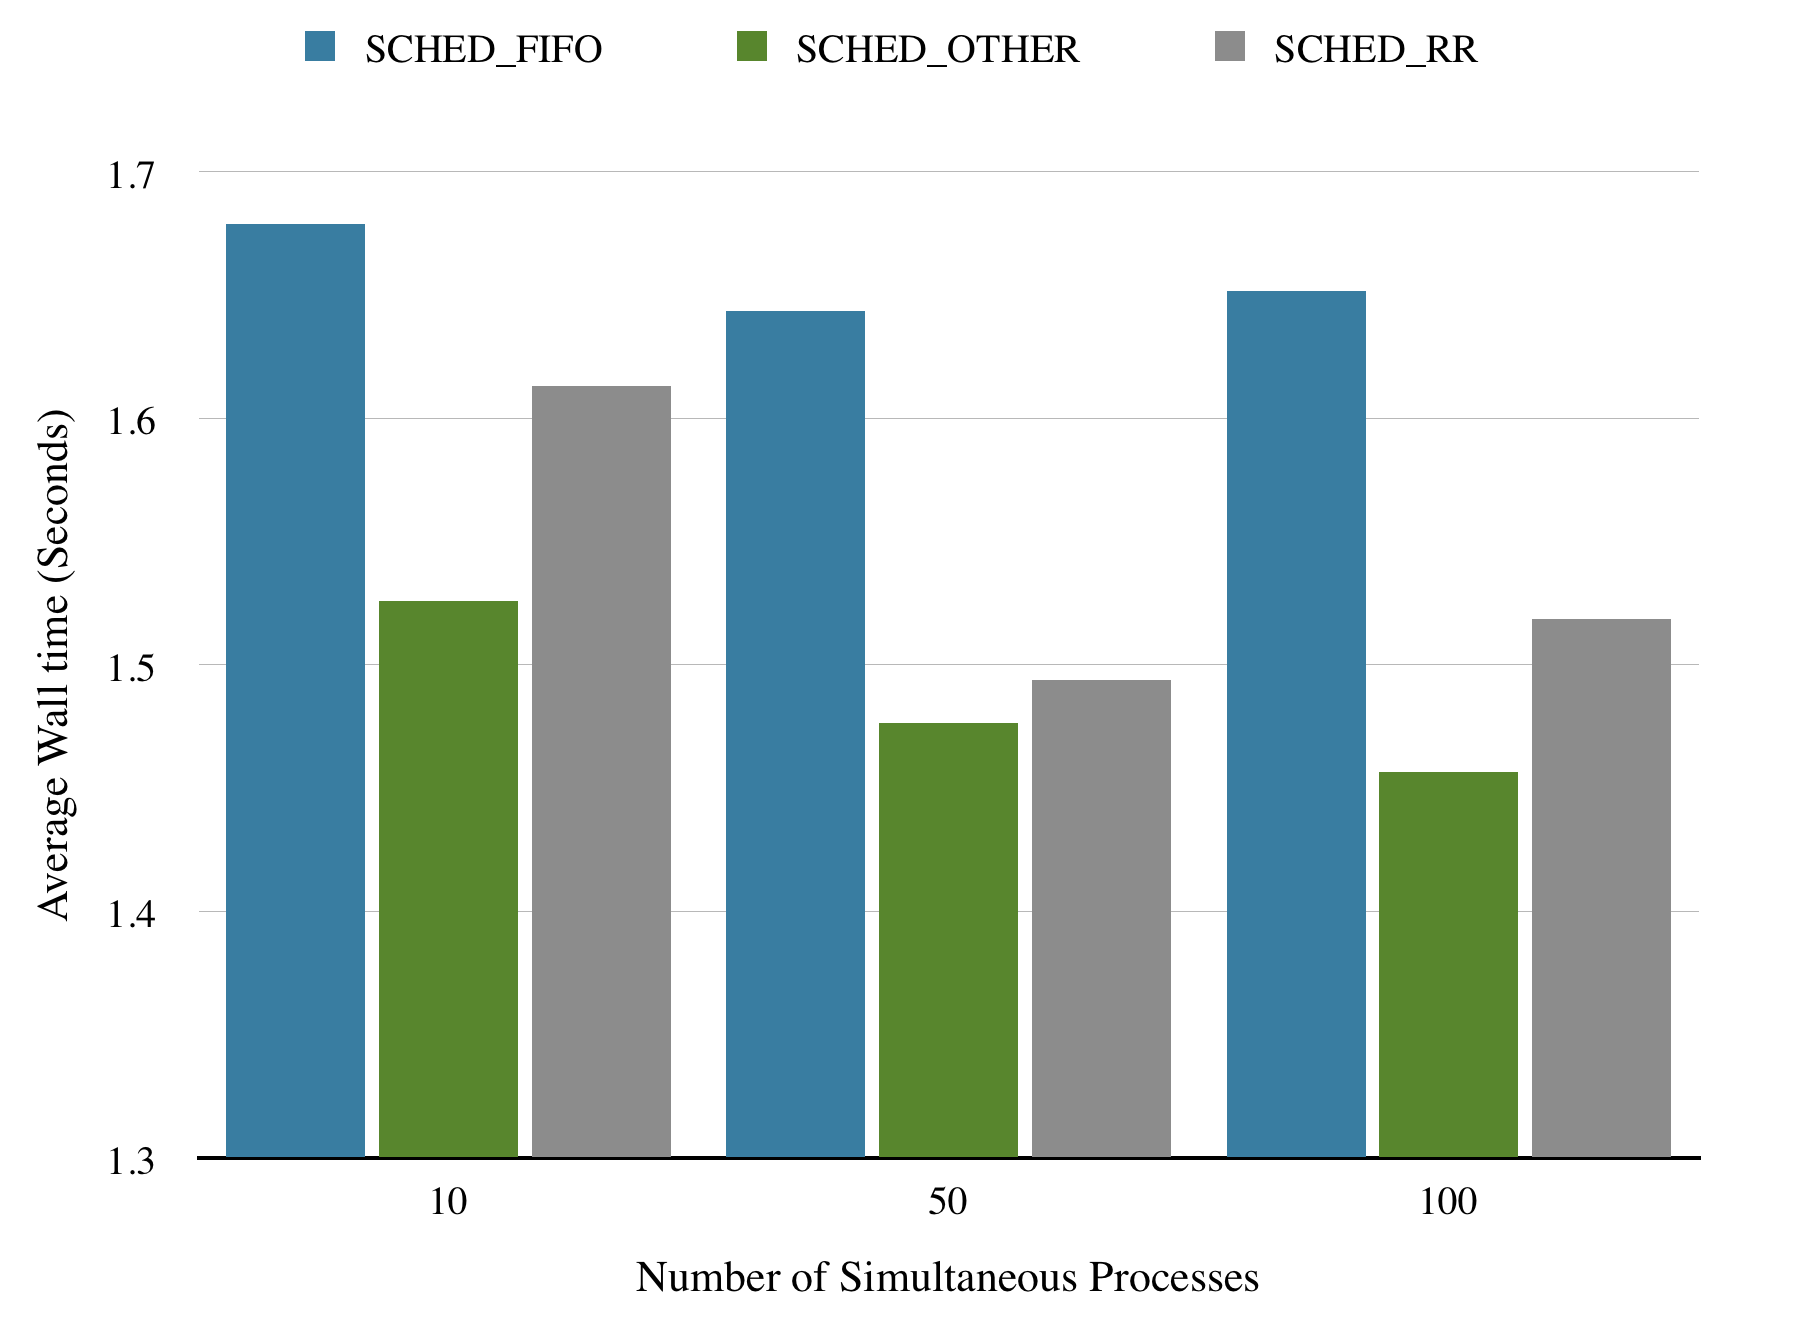
\includegraphics[width=100mm]{CPUWall.png}
    \caption{Wall time for the CPU bound benchmark}
    \label{fig:cpuwall}
  \end{center} 
\end{figure}

Figure~\ref{fig:cpuwall} shows the results for the wall time of the CPU bound
benchmark {\ttfamily pi-sched.c}. The results indicate that {\ttfamily SCHED\_
OTHER} is the best scheduler with regard to wall time, as in all three cases
of forking 10, 50, and 100 times the benchmarks being run according to the 
{\ttfamily SCHED\_OTHER} scheduler finished with the shortest wall time. This 
result indicates that the CFS is the best way to handle processes that are CPU
bound

\begin{figure}[!htb]
  \begin{center}
    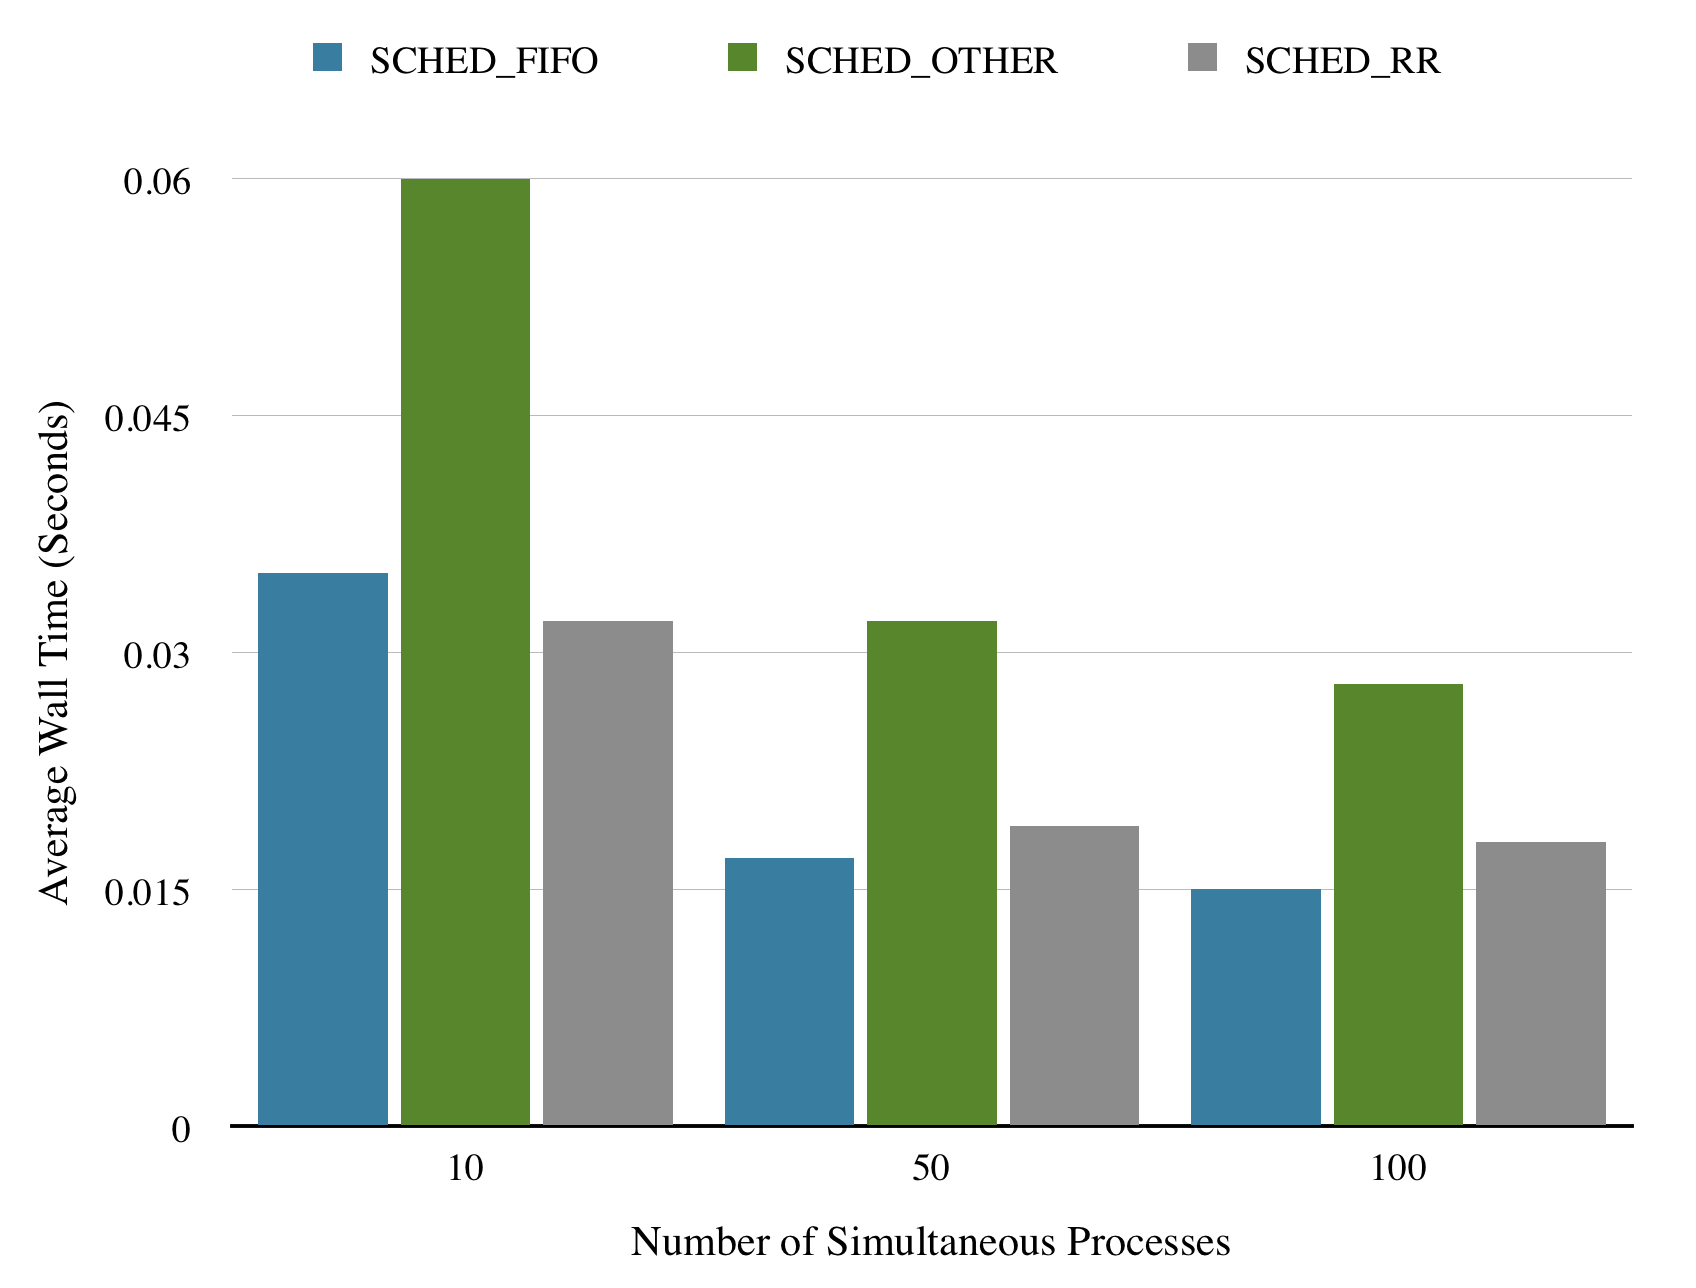
\includegraphics[width=100mm]{IOWall.png}
    \caption{Wall time for the I/O bound benchmark}
    \label{fig:iowall}
  \end{center} 
\end{figure}

Figure~\ref{fig:iowall} shows the wall times for the I/O bound benchmark 
{\ttfamily rw-sched.c}. Clearly, in this case, {\ttfamily SCHED\_OTHER} is the
worst scheduler with regard to wall time, since the wall time is nearly double
the wall time of the other two schedulers. However, the difference between 
using {\ttfamily SCHED\_RR} and {\ttfamily SCHED\_FIFO} seems to be negligible,
since with 10 simultaneous processes {\ttfamily SCHED\_RR} appears to be slightly
faster with regard to wall time, but with more number of simultaneous processes,
{\ttfamily SCHED\_FIFO} appears to be slightly faster. 

\begin{figure}[!htb]
  \centering
  \begin{subfigure}[t]{0.4\textwidth}
    \centering
    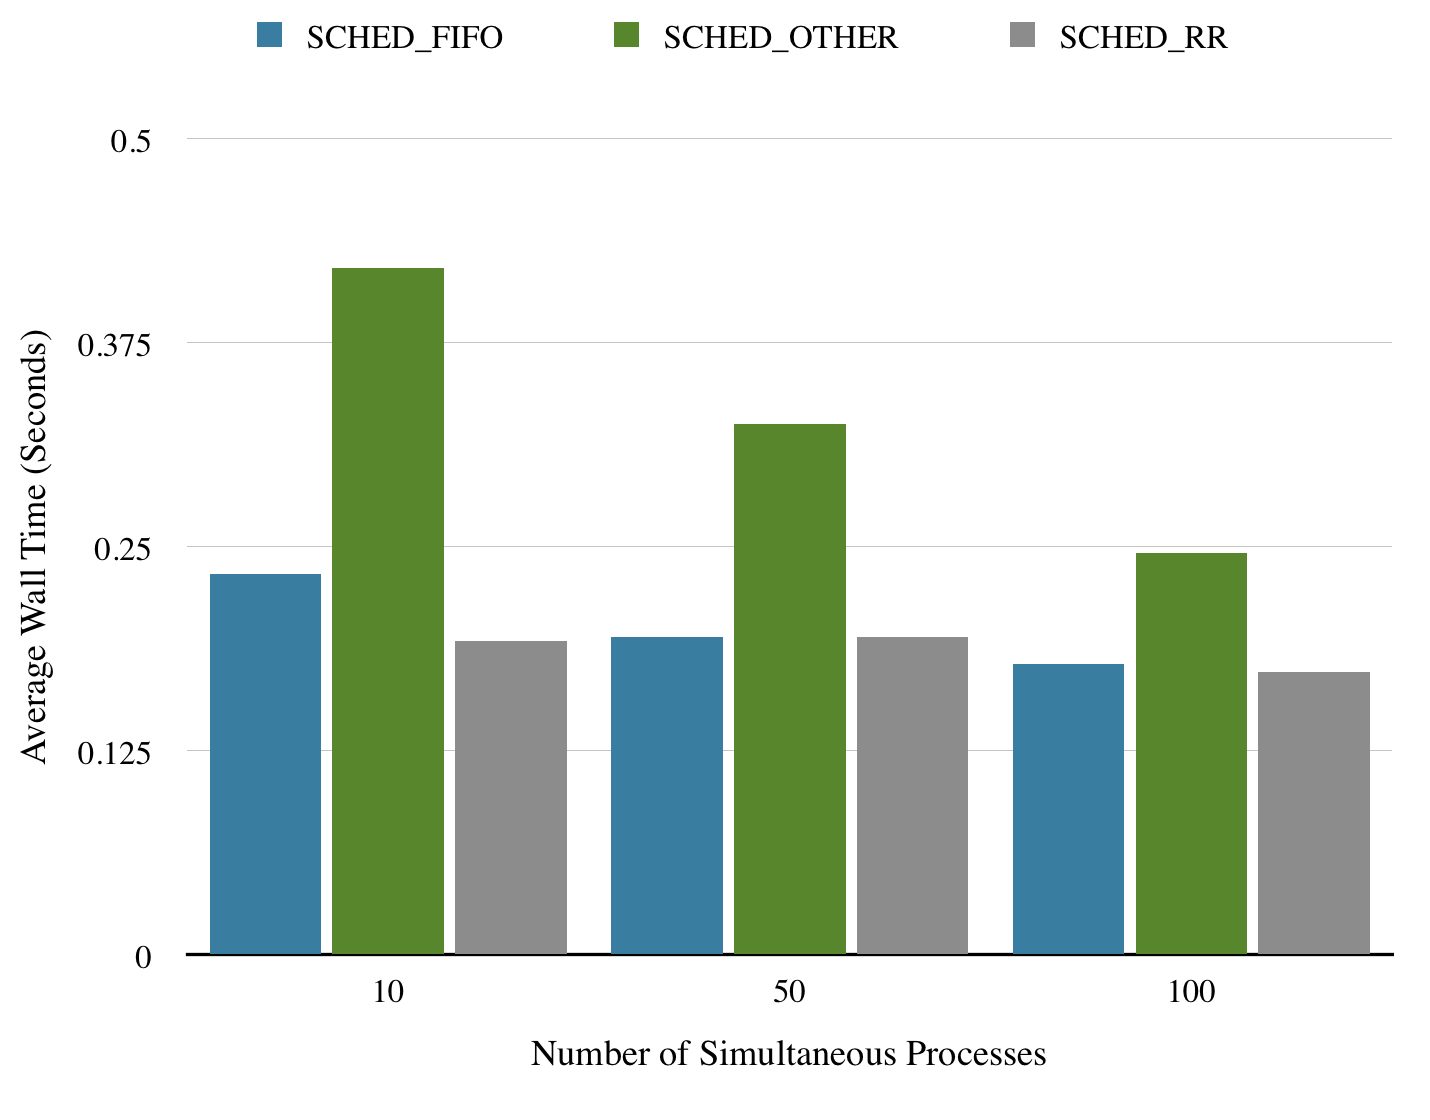
\includegraphics[width=75mm]{MixedWall.png}
    \caption{Wall time for the mixed benchmark}
    \label{fig:mixwall}
  \end{subfigure}
  ~
  \begin{subfigure}[t]{0.4\textwidth}
    \centering
    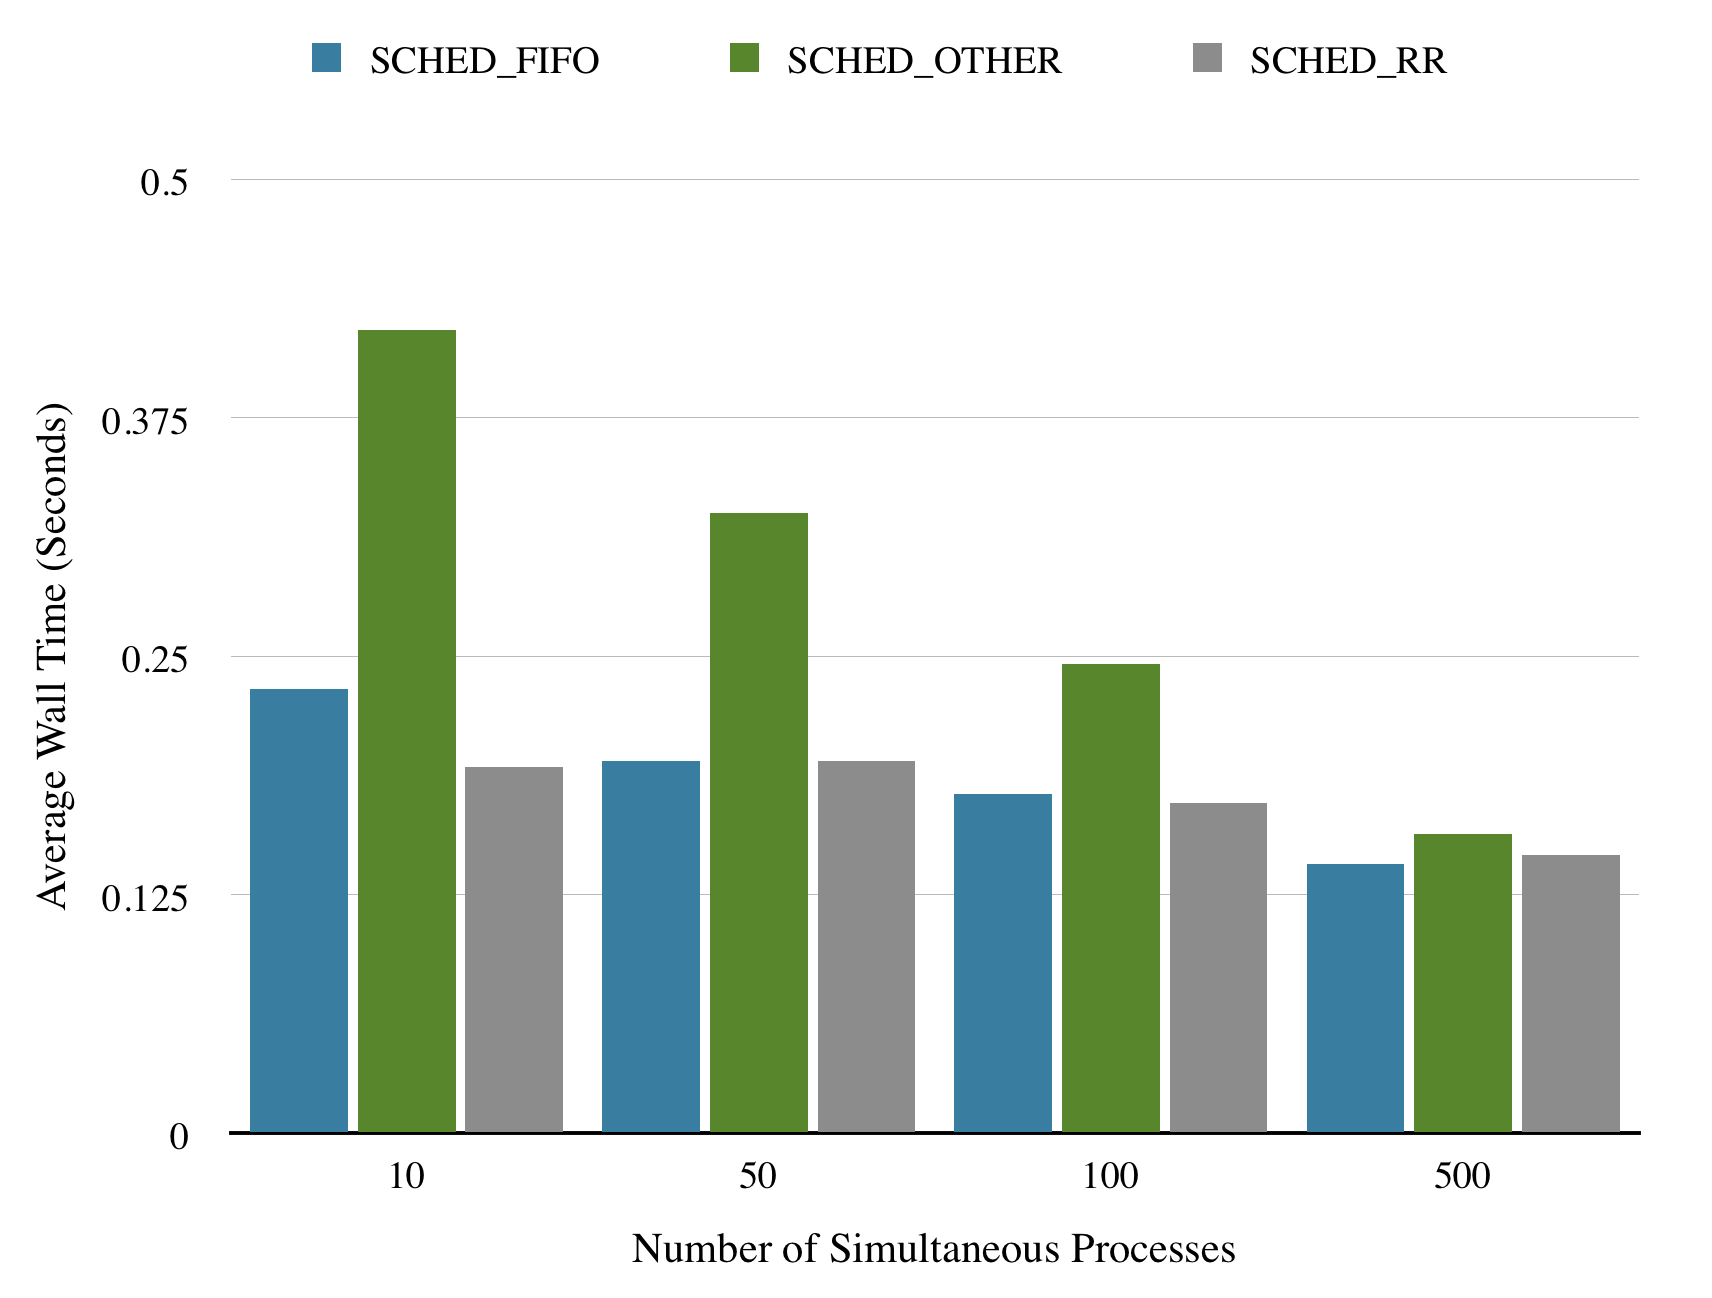
\includegraphics[width=75mm]{MixWallMore.png}
    \caption{Wall time for the mixed benchmark, with 500 processes}
    \label{fig:mixwallmore}
  \end{subfigure}
  \caption{Wall times for mixed benchmark}
\end{figure}

Finally, Figure~\ref{fig:mixwall} shows the wall times for the mixed benchmark
{\ttfamily mix-sched.c}. The results here seem to be similar to the results for
the I/O bound benchmark, in that {\ttfamily SCHED\_OTHER} appears to be the 
worst scheduling policy, with both other real-time schedulers giving much better
performance with regard to wall time. However, the performance difference 
between {\ttfamily SCHED\_OTHER} and both of the real-time schedulers is 
decreasing as the number of simultaneous processes increases.

By collecting additional data for 500 simultaneous processes (Appendix A:
Additional Data), Figure~\ref{fig:mixwallmore} was generated. This shows that as
the number of simultaneous processes increases, all three scheduling algorithms
become more equal with neither having a clear advantage over the other.

\subsection{Context Switches}
The number of context switches also describe how each of the scheduling 
algorithms runs. By examining the graphs of context switched, it is clear that
{\ttfamily SCHED\_OTHER} causes an increase in both voluntary and involuntary
context switches in all of the benchmarks run, most likely due to how the
algorithm will preempt a running process once that process's time slice has been
used up.

\begin{figure}[!htb]
  \centering
  \begin{subfigure}[t]{0.4\textwidth}
    \centering
    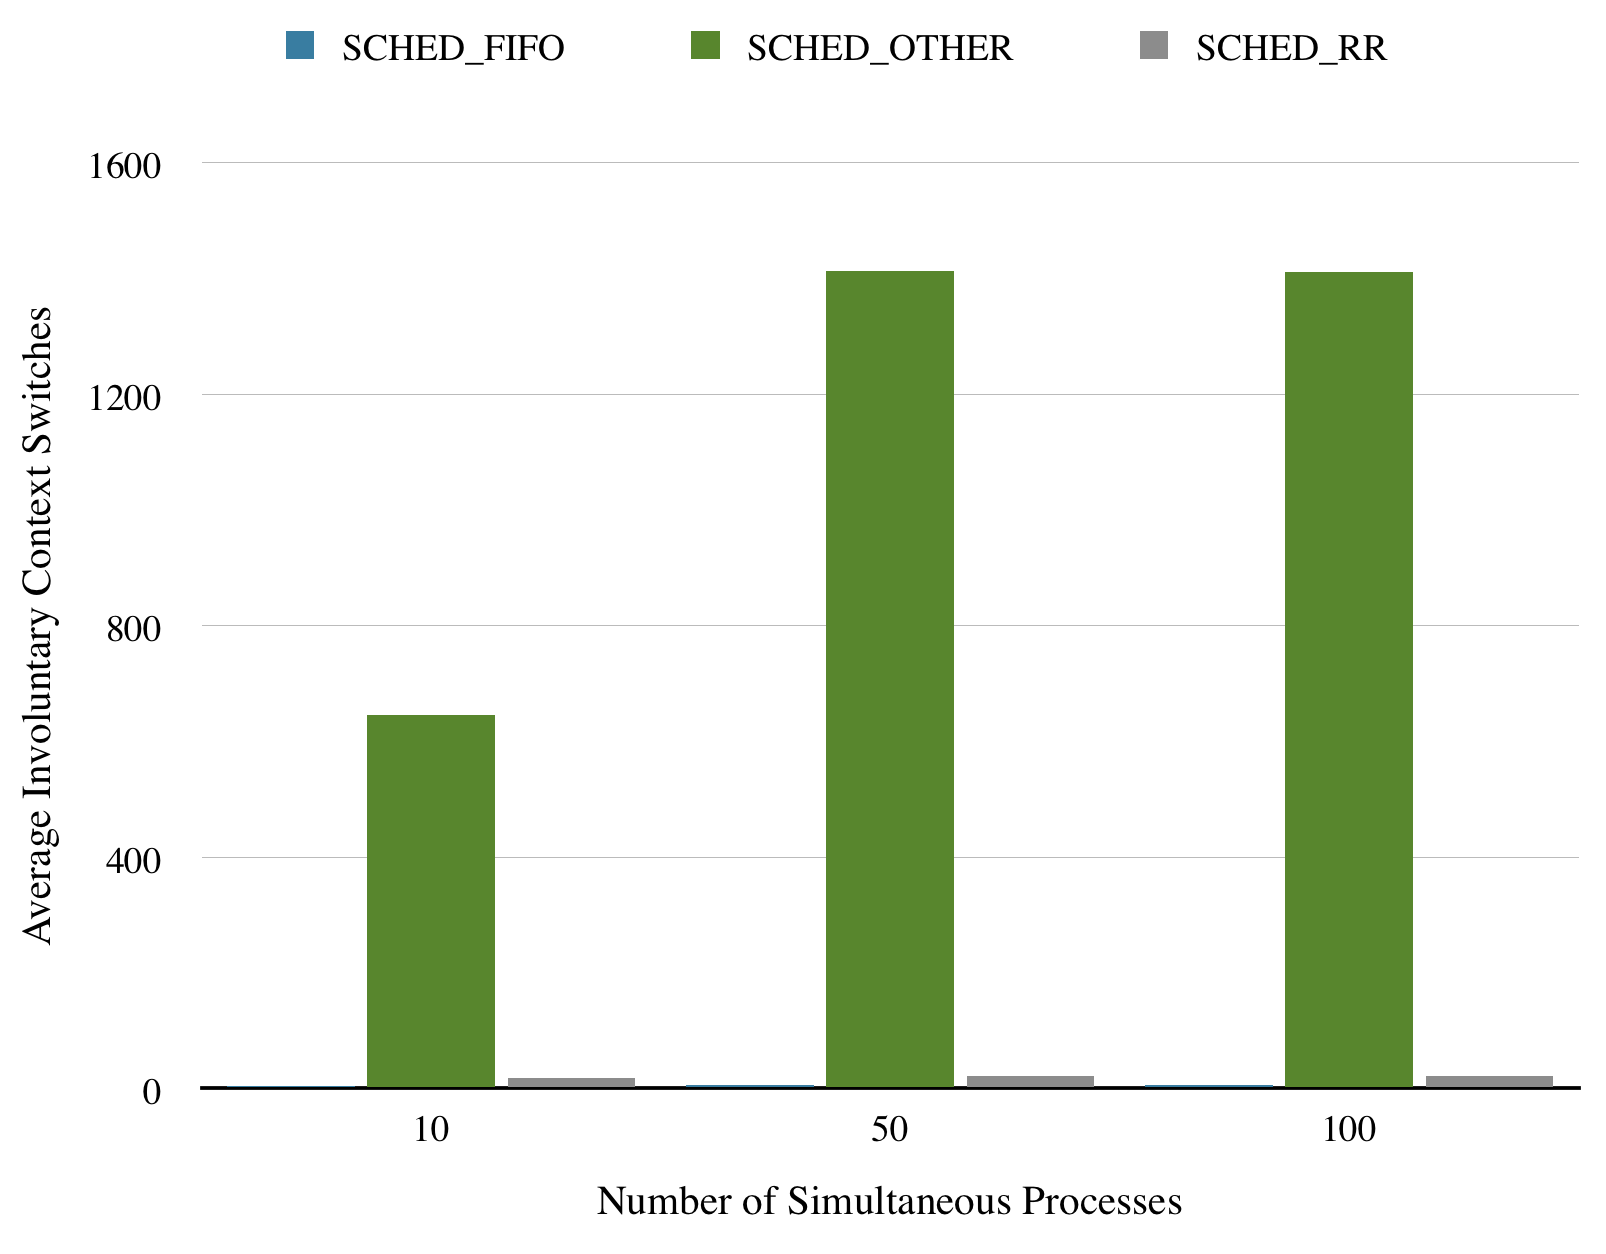
\includegraphics[width=75mm]{CPUIC.png}
    \caption{Involuntary context switches}
    \label{fig:cpuic}
  \end{subfigure}
  ~
  \begin{subfigure}[t]{0.4\textwidth}
    \centering
    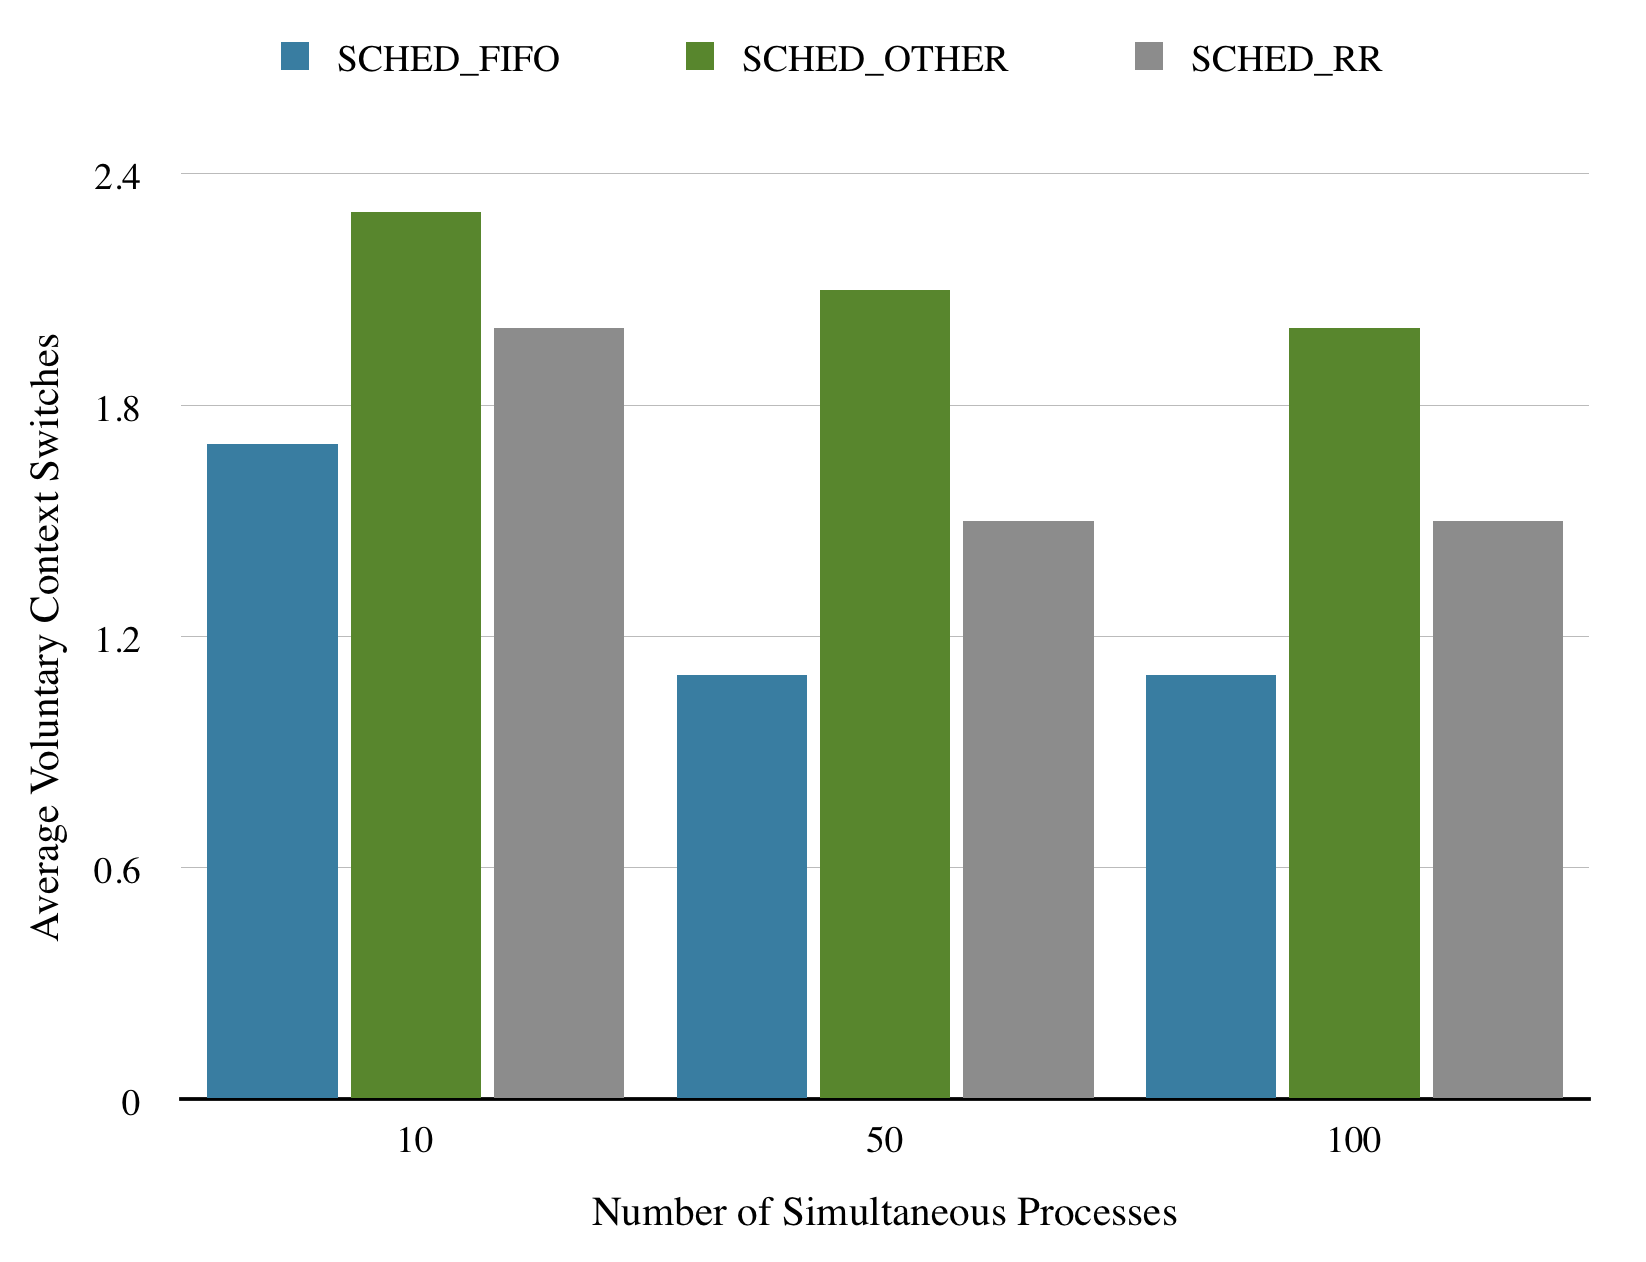
\includegraphics[width=75mm]{CPUVC.png}
    \caption{Voluntary context switches}
    \label{fig:cpuvc}
  \end{subfigure}
  \caption{Context switched for a CPU bound process}
\end{figure}

\begin{figure}[!htb]
  \centering
  \begin{subfigure}[t]{0.4\textwidth}
    \centering
    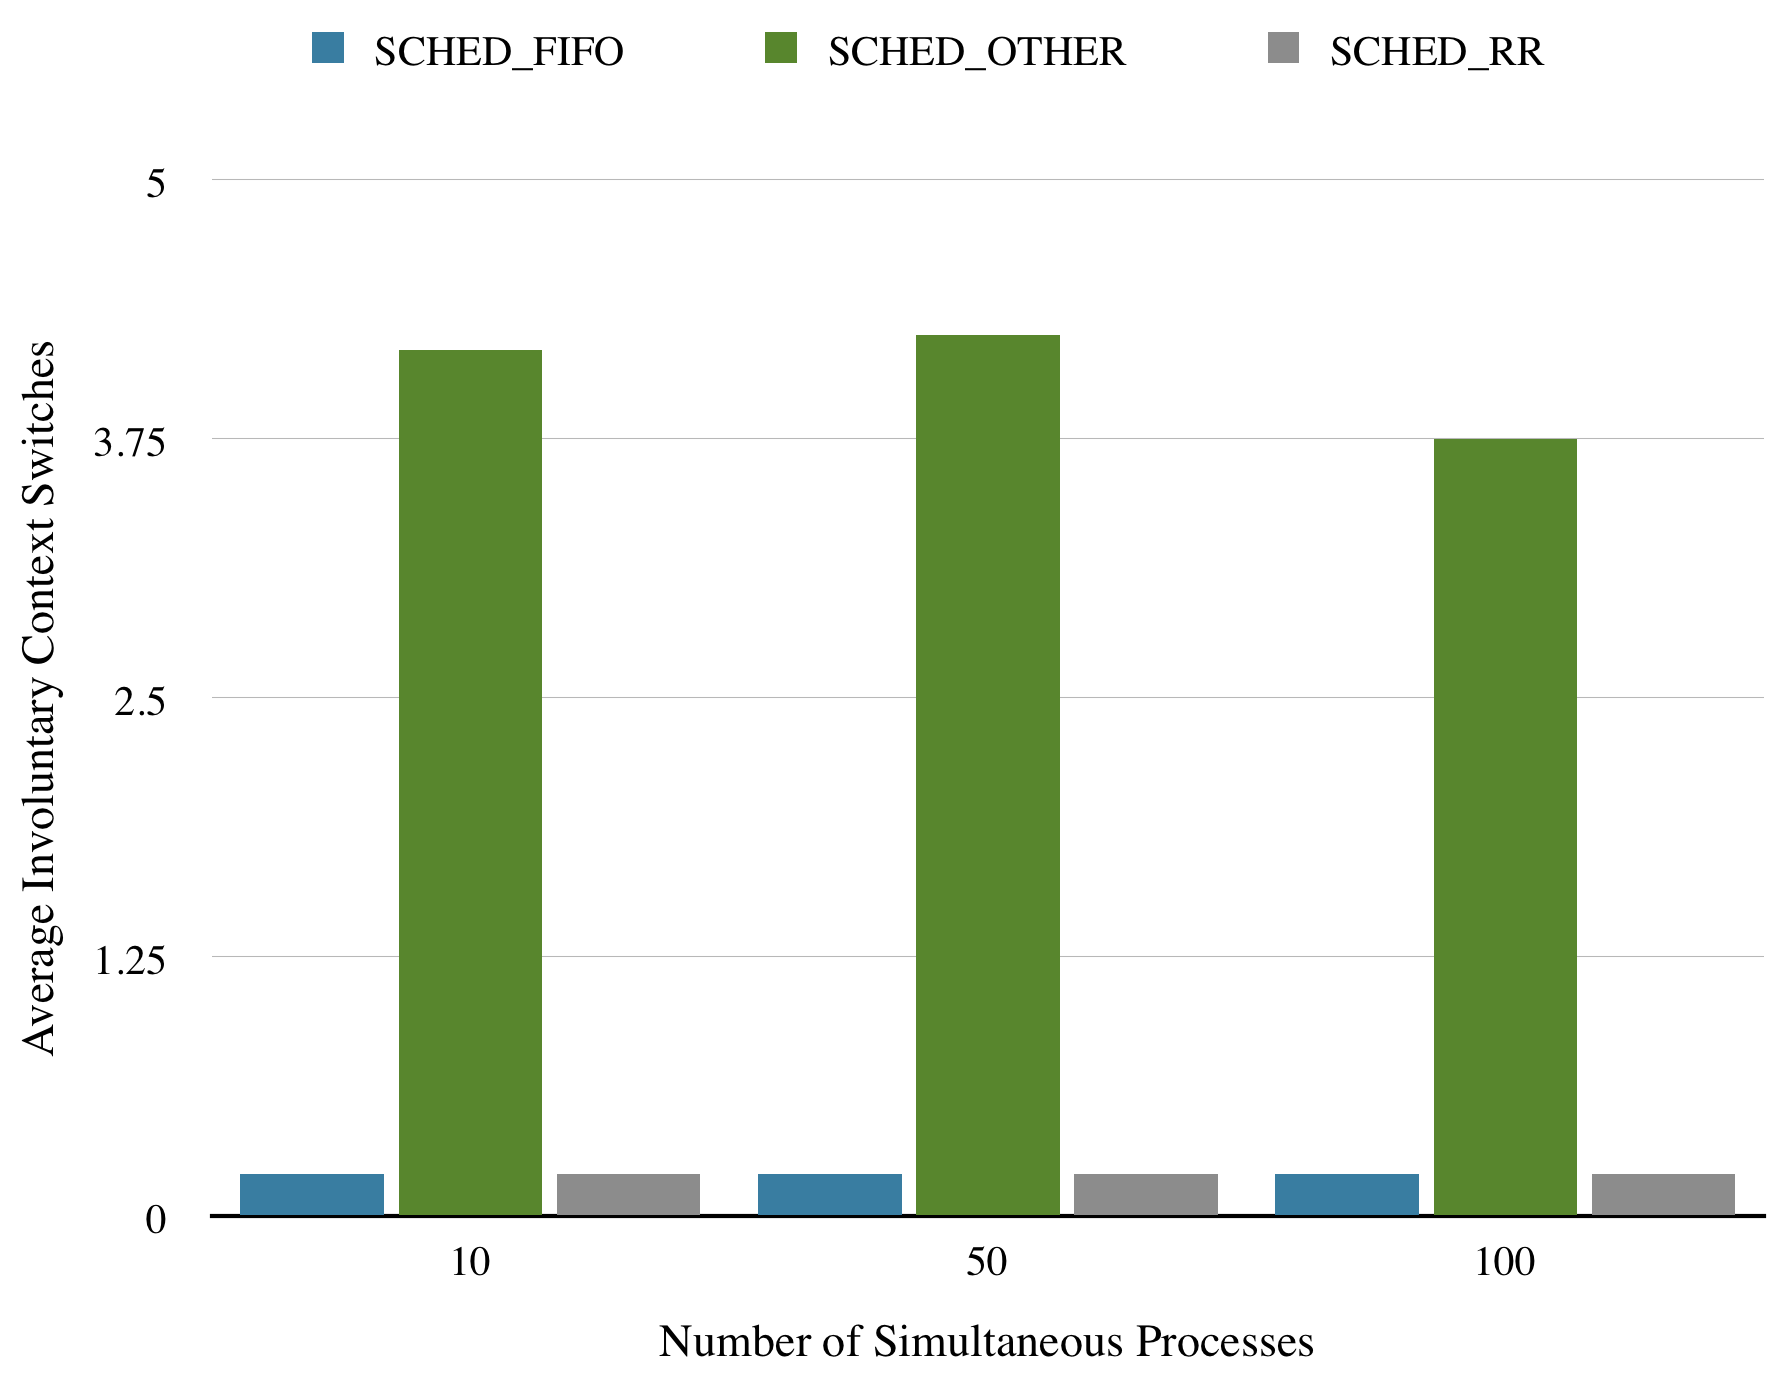
\includegraphics[width=75mm]{IOIC.png}
    \caption{Involuntary context switches}
    \label{fig:ioic}
  \end{subfigure}
  ~
  \begin{subfigure}[t]{0.4\textwidth}
    \centering
    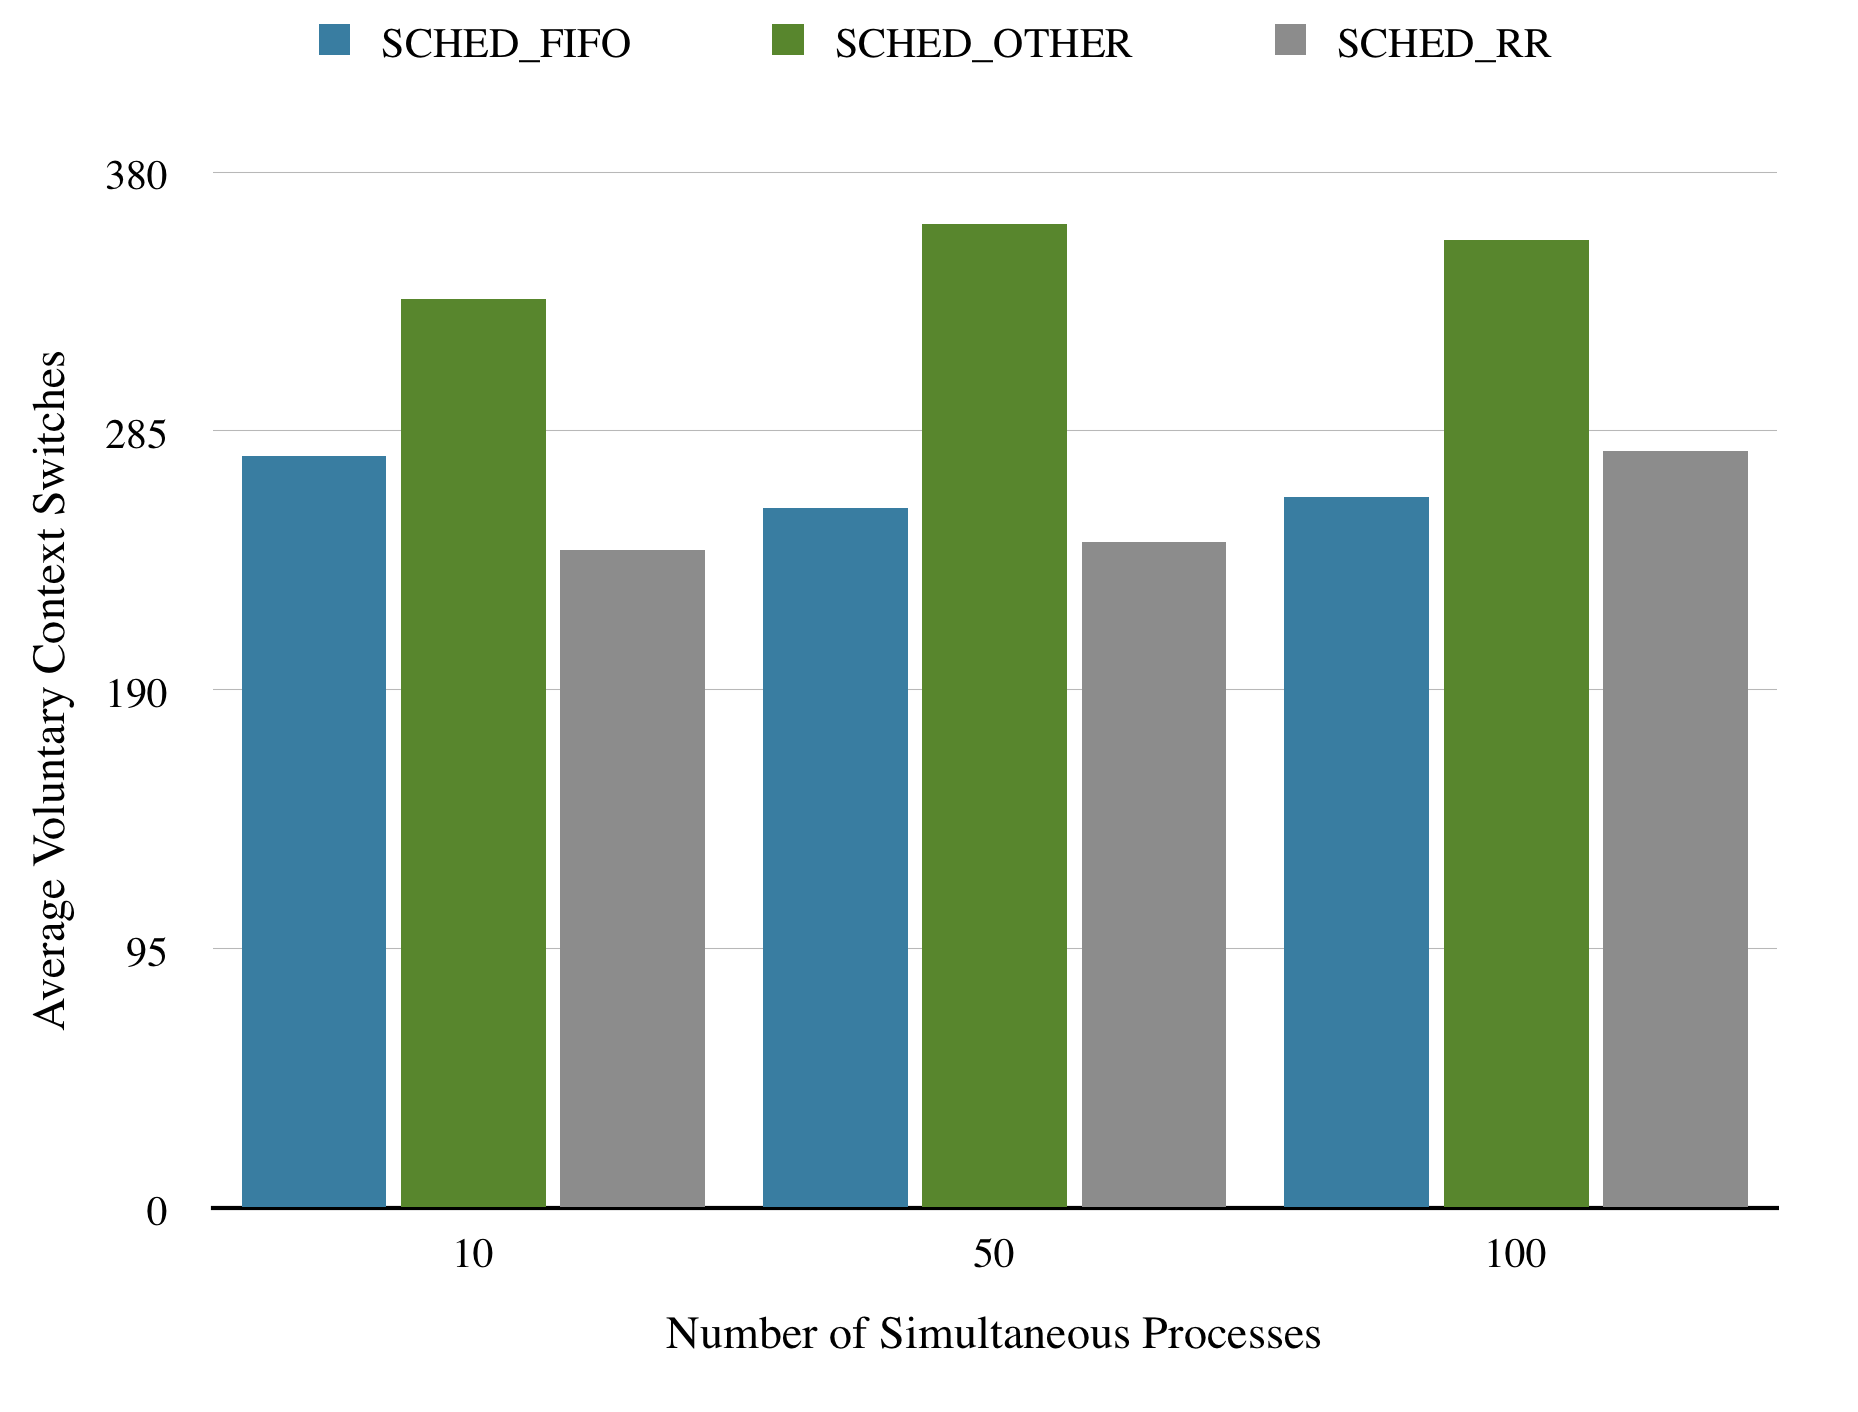
\includegraphics[width=75mm]{IOVC.png}
    \caption{Voluntary context switches}
    \label{fig:iovc}
  \end{subfigure}
  \caption{Context switched for a I/O bound process}
\end{figure}

\begin{figure}[!htb]
  \centering
  \begin{subfigure}[t]{0.4\textwidth}
    \centering
    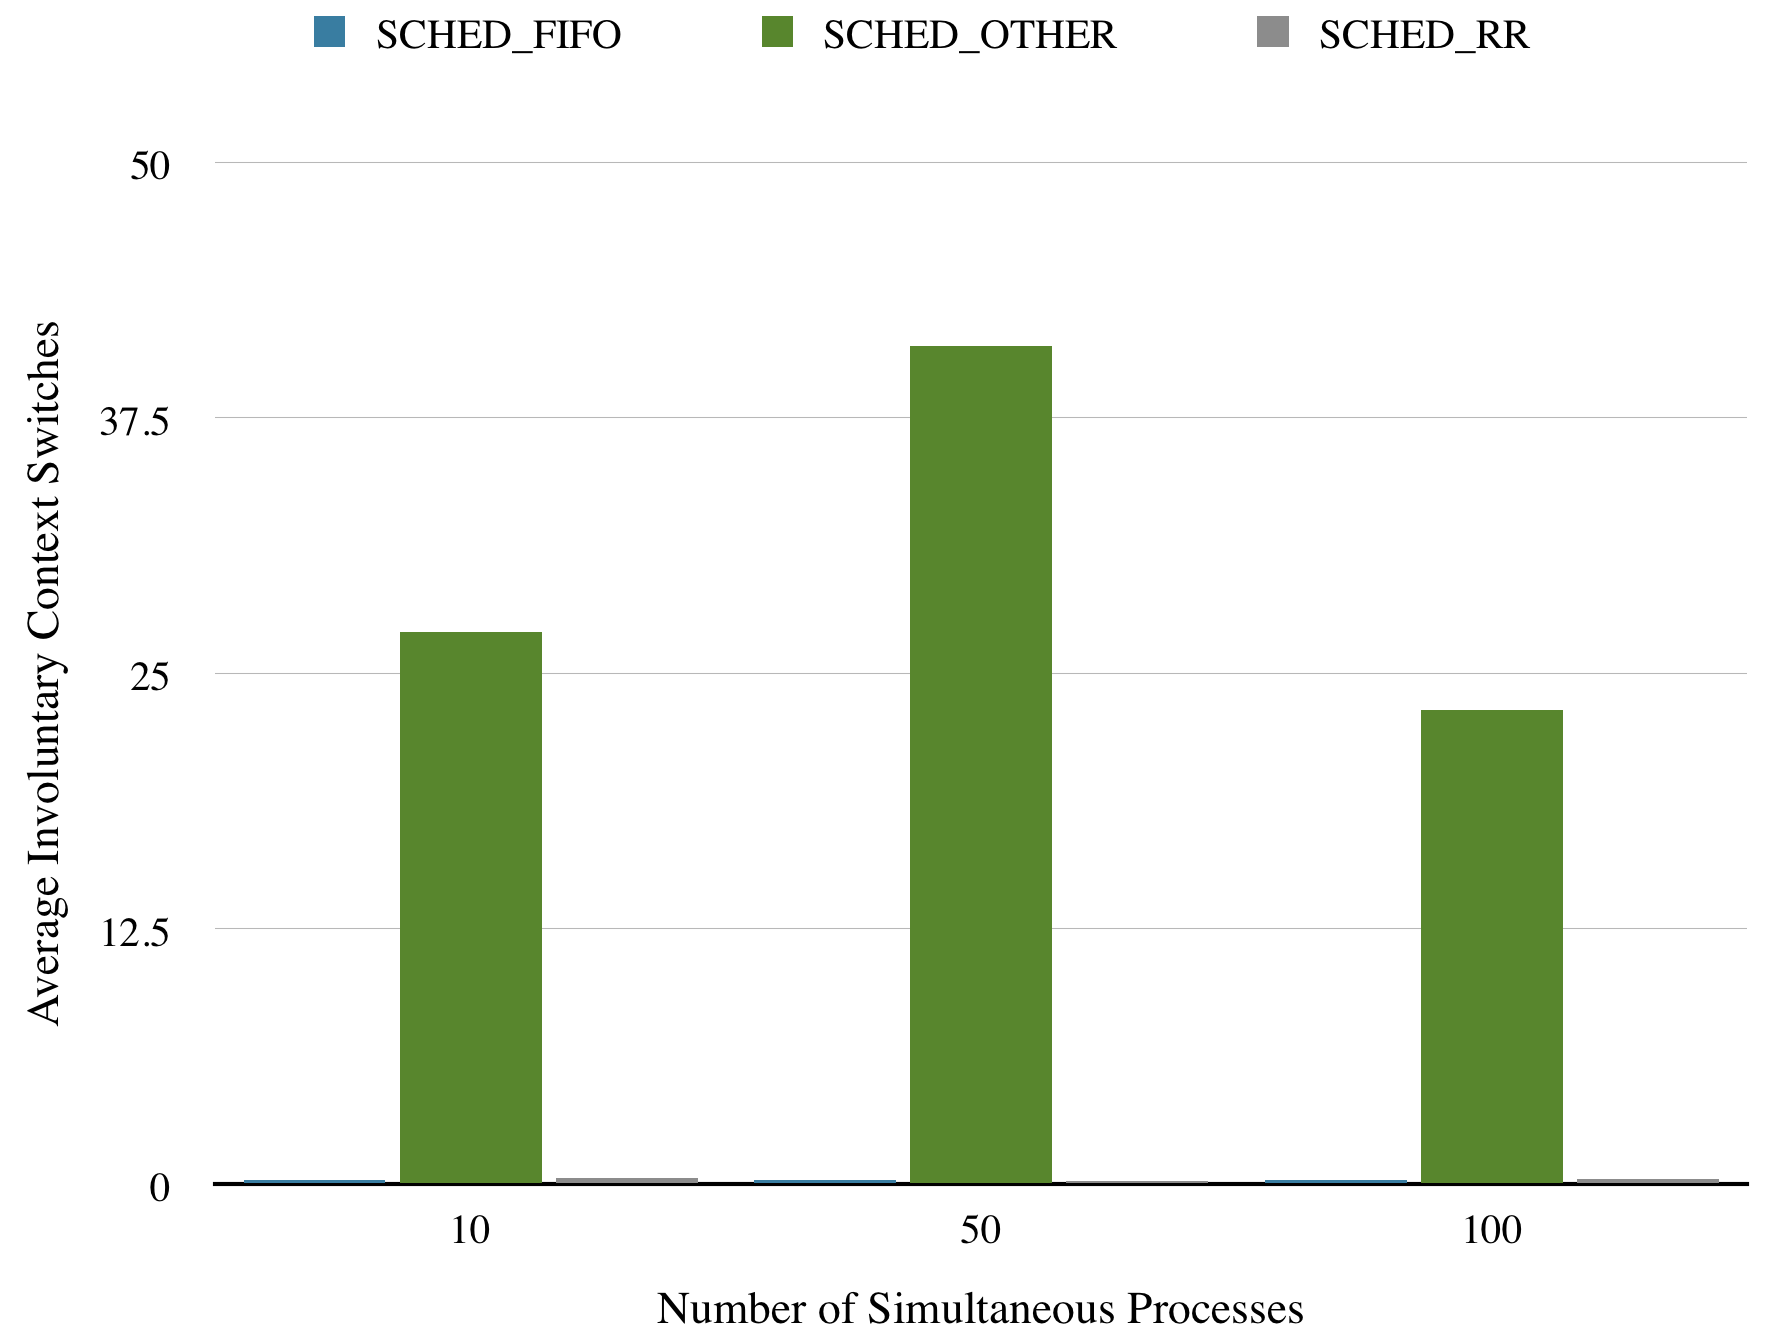
\includegraphics[width=75mm]{MixIC.png}
    \caption{Involuntary context switches}
    \label{fig:mixic}
  \end{subfigure}
  ~
  \begin{subfigure}[t]{0.4\textwidth}
    \centering
    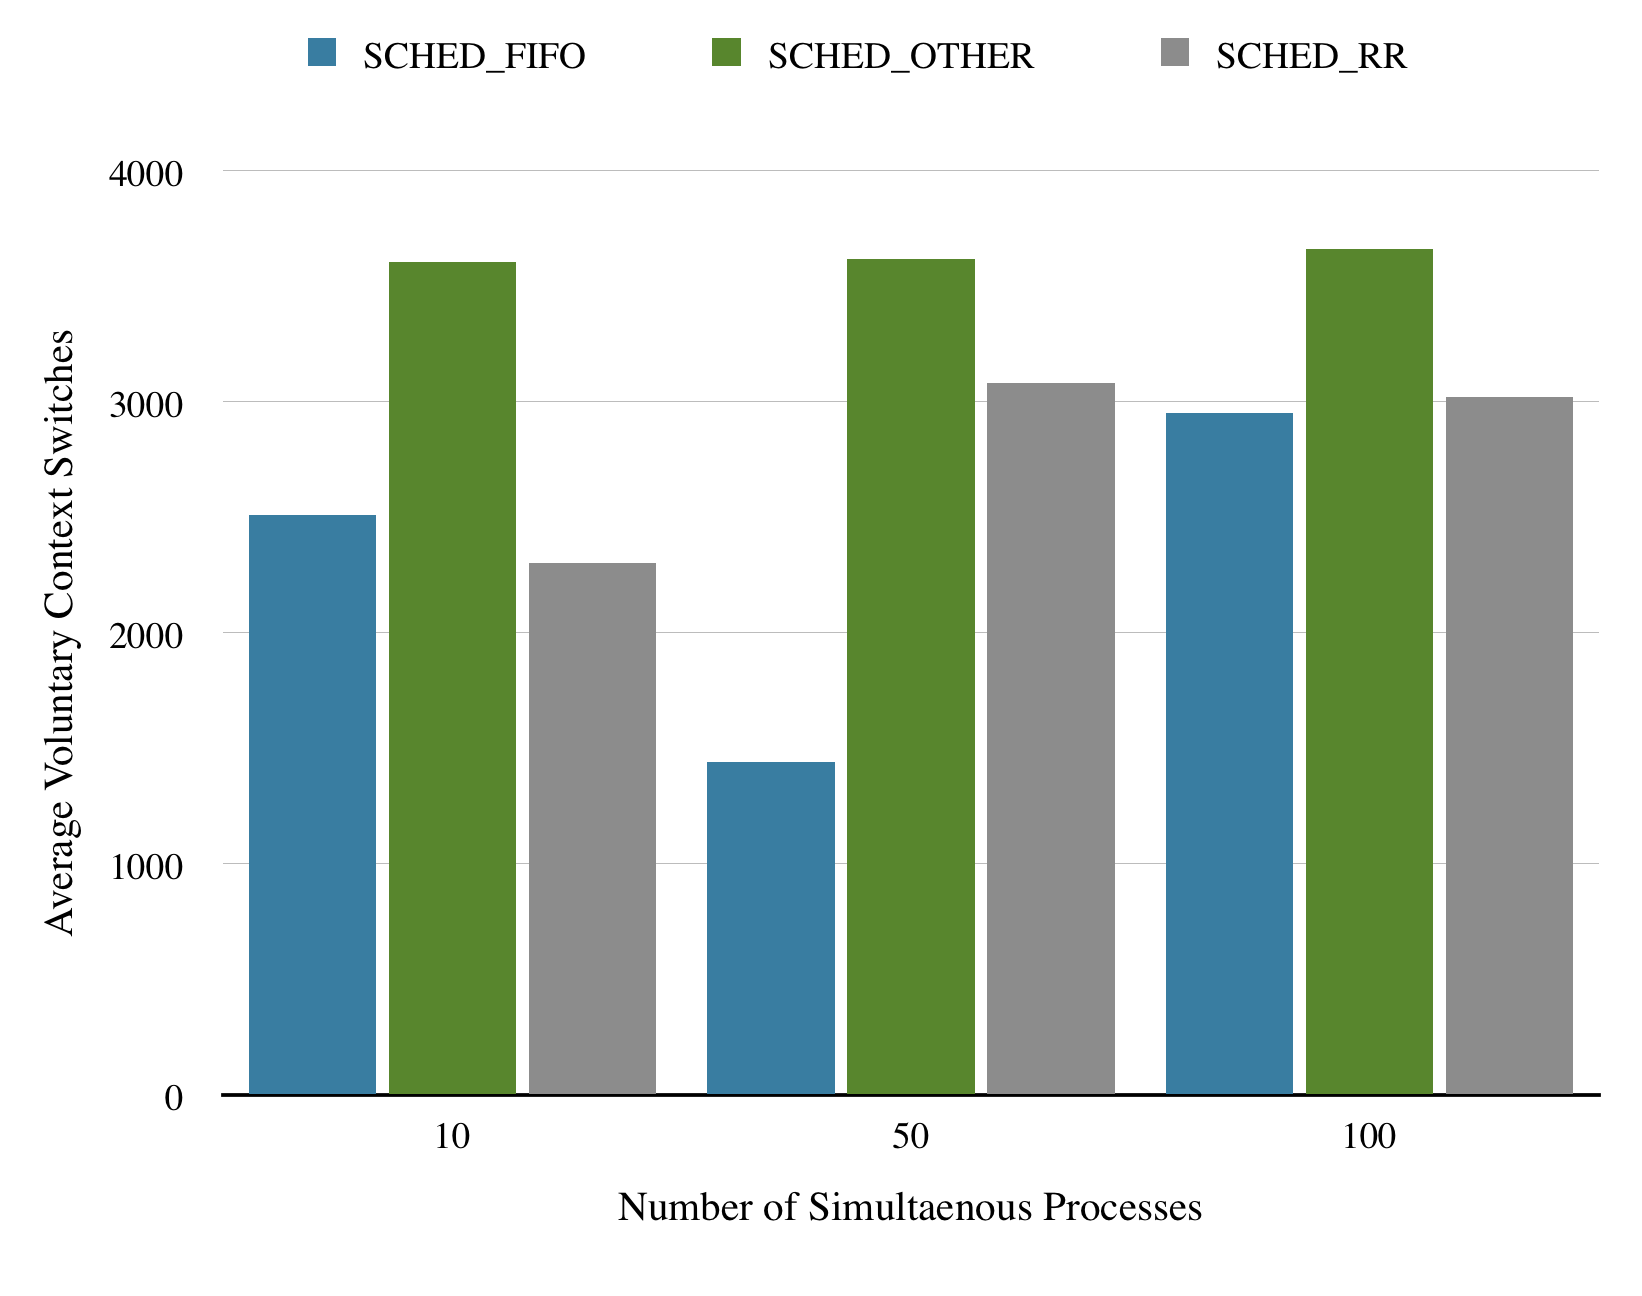
\includegraphics[width=75mm]{MixVC.png}
    \caption{Voluntary context switches}
    \label{fig:mixvc}
  \end{subfigure}
  \caption{Context switched for a mixed process}
\end{figure}

As the {\ttfamily SCHED\_OTHER} algorithm runs by allocating each of the 
processes a given time slice, it is also most likely to preempt a process if
that process has not blocked by the end of its time slice. Thus, the amount
of involuntary context switches for a CPU bound process is much higher than
that of an I/O bound process, as can be seen by comparing Figure~\ref{fig:cpuic}
and Figure~\ref{fig:ioic}. While there are not as many involuntary context
switches for the mixed program (Figure~\ref{fig:mixic}), the number of 
involuntary context switches is still higher than that of the I/O bound program.
Both of the real-time scheduling algorithms, {\ttfamily SCHED\_RR} and 
{\ttfamily SCHED\_FIFO} do not preempt the running processes nearly as much as
{\ttfamily SCHED\_OTHER}.


\section{Conclusion}

Overall, it is evident that the different scheduling algorithms are suited to
different tasks. If a program is CPU bound, then CFS algorithms such as 
{\ttfamily SCHED\_OTHER} present a clear performance advantage when looking the
wall time of the program. On the other hand, if a process is I/O bound, then 
the real-time scheduling algorithms such as {\ttfamily SCHED\_RR} and 
{\ttfamily SCHED\_FIFO} are generally faster when comparing wall times to a 
CFS algorithm. However, the distinction becomes less clear when a process is
neither CPU nor I/O bound, and is instead mixed. Then. if the number of 
simultaneous processes is low, the real-time algorithms are still at an 
advantage when compared to the CFS algorithm, but as the number of simultaneous
processes increases, the advantage disappears and both real-time and CFS 
algorithms present similar wall time performance


\newpage

\section{Appendix A: Data}
Raw data collected from running the test scripts, and additional data for 
{\ttfamily mix-sched.c}.

\subsection{Initial Data Collection}
\begin{small}
\begin{verbatim}
Testing CPU Intensive Process
Calculating pi over 100000000 iterations using SCHED_FIFO with 10 simultaneous processes...
wall=17.34 user=50.66 system=0.15 CPU=292% i-switched=44 v-switched=17
wall=16.95 user=51.84 system=0.22 CPU=307% i-switched=42 v-switched=17
wall=16.61 user=53.79 system=0.21 CPU=325% i-switched=47 v-switched=17
wall=16.10 user=53.69 system=0.22 CPU=334% i-switched=46 v-switched=17
wall=16.93 user=57.53 system=0.34 CPU=341% i-switched=51 v-switched=17

Calculating pi over 100000000 iterations using SCHED_FIFO with 50 simultaneous processes...
wall=86.76 user=314.41 system=1.80 CPU=364% i-switched=319 v-switched=57
wall=83.57 user=310.08 system=1.71 CPU=373% i-switched=315 v-switched=57
wall=77.12 user=284.33 system=1.28 CPU=370% i-switched=286 v-switched=57
wall=88.08 user=316.75 system=1.01 CPU=360% i-switched=322 v-switched=57
wall=78.38 user=277.94 system=1.10 CPU=356% i-switched=278 v-switched=57

Calculating pi over 100000000 iterations using SCHED_FIFO with 100 simultaneous processes...
wall=172.38 user=643.74 system=3.27 CPU=375% i-switched=671 v-switched=107
wall=180.28 user=673.82 system=2.68 CPU=375% i-switched=702 v-switched=107
wall=177.01 user=664.32 system=2.53 CPU=376% i-switched=690 v-switched=107
wall=148.02 user=549.93 system=2.48 CPU=373% i-switched=571 v-switched=107
wall=148.01 user=550.18 system=2.32 CPU=373% i-switched=566 v-switched=107

Calculating pi over 100000000 iterations using SCHED_OTHER with 10 simultaneous processes...
wall=14.28 user=56.26 system=0.24 CPU=395% i-switched=5961 v-switched=23
wall=14.79 user=58.03 system=0.23 CPU=393% i-switched=6348 v-switched=23
wall=14.43 user=56.85 system=0.20 CPU=395% i-switched=6153 v-switched=22
wall=16.20 user=63.19 system=0.42 CPU=392% i-switched=6637 v-switched=23
wall=16.59 user=64.73 system=0.55 CPU=393% i-switched=6661 v-switched=23

Calculating pi over 100000000 iterations using SCHED_OTHER with 50 simultaneous processes...
wall=71.86 user=284.99 system=0.84 CPU=397% i-switched=69536 v-switched=103
wall=69.73 user=276.94 system=0.64 CPU=398% i-switched=68530 v-switched=103
wall=72.08 user=285.90 system=0.73 CPU=397% i-switched=70559 v-switched=103
wall=77.60 user=306.61 system=1.34 CPU=396% i-switched=72851 v-switched=103
wall=76.83 user=303.18 system=1.44 CPU=396% i-switched=72033 v-switched=103

Calculating pi over 100000000 iterations using SCHED_OTHER with 100 simultaneous processes...
wall=143.74 user=570.52 system=1.45 CPU=397% i-switched=141154 v-switched=202
wall=154.60 user=610.72 system=2.68 CPU=396% i-switched=144952 v-switched=203
wall=149.70 user=592.16 system=2.31 CPU=397% i-switched=142460 v-switched=203
wall=139.90 user=556.29 system=1.07 CPU=398% i-switched=138225 v-switched=203
wall=140.20 user=557.44 system=1.06 CPU=398% i-switched=138606 v-switched=203

Calculating pi over 100000000 iterations using SCHED_RR with 10 simultaneous processes...
wall=16.48 user=54.49 system=0.20 CPU=331% i-switched=188 v-switched=20
wall=15.86 user=53.52 system=0.24 CPU=338% i-switched=180 v-switched=19
wall=15.95 user=53.42 system=0.22 CPU=336% i-switched=180 v-switched=19
wall=16.04 user=53.70 system=0.19 CPU=336% i-switched=186 v-switched=21
wall=16.32 user=54.90 system=0.19 CPU=337% i-switched=182 v-switched=19

Calculating pi over 100000000 iterations using SCHED_RR with 50 simultaneous processes...
wall=74.71 user=276.04 system=1.26 CPU=371% i-switched=1038 v-switched=72
wall=74.74 user=272.94 system=1.22 CPU=366% i-switched=1039 v-switched=79
wall=74.03 user=277.63 system=1.19 CPU=376% i-switched=1029 v-switched=75
wall=74.92 user=275.72 system=1.28 CPU=369% i-switched=1042 v-switched=78
wall=75.01 user=272.88 system=1.28 CPU=365% i-switched=1035 v-switched=76

Calculating pi over 100000000 iterations using SCHED_RR with 100 simultaneous processes...
wall=152.85 user=577.31 system=1.78 CPU=378% i-switched=2186 v-switched=162
wall=155.04 user=580.66 system=2.03 CPU=375% i-switched=2177 v-switched=170
wall=153.90 user=581.39 system=2.00 CPU=379% i-switched=2160 v-switched=139
wall=149.66 user=559.15 system=1.80 CPU=374% i-switched=2004 v-switched=135
wall=147.74 user=555.54 system=2.59 CPU=377% i-switched=1984 v-switched=159

============================
Testing I/O Intensive Process
Reading and writing using SCHED_FIFO with 10 simultaneous processes...
wall=0.39 user=0.00 system=0.12 CPU=31% i-switched=2 v-switched=2928
wall=0.39 user=0.00 system=0.08 CPU=23% i-switched=2 v-switched=2990
wall=0.50 user=0.00 system=0.10 CPU=22% i-switched=2 v-switched=3830
wall=0.24 user=0.00 system=0.05 CPU=24% i-switched=2 v-switched=2017
wall=0.25 user=0.00 system=0.05 CPU=25% i-switched=2 v-switched=2031

Reading and writing using SCHED_FIFO with 50 simultaneous processes...
wall=1.13 user=0.05 system=0.18 CPU=20% i-switched=2 v-switched=16339
wall=0.90 user=0.05 system=0.18 CPU=26% i-switched=2 v-switched=10322
wall=0.91 user=0.03 system=0.20 CPU=26% i-switched=2 v-switched=10300
wall=0.82 user=0.04 system=0.18 CPU=27% i-switched=2 v-switched=10087
wall=1.30 user=0.06 system=0.15 CPU=16% i-switched=2 v-switched=17177

Reading and writing using SCHED_FIFO with 100 simultaneous processes...
wall=1.41 user=0.08 system=0.36 CPU=31% i-switched=2 v-switched=22632
wall=1.37 user=0.07 system=0.38 CPU=33% i-switched=2 v-switched=22643
wall=1.39 user=0.06 system=0.38 CPU=31% i-switched=2 v-switched=24015
wall=1.87 user=0.04 system=0.80 CPU=45% i-switched=2 v-switched=29981
wall=1.85 user=0.06 system=0.92 CPU=52% i-switched=2 v-switched=31203

Reading and writing using SCHED_OTHER with 10 simultaneous processes...
wall=0.75 user=0.00 system=0.56 CPU=75% i-switched=47 v-switched=3482
wall=0.62 user=0.00 system=0.41 CPU=66% i-switched=19 v-switched=3681
wall=0.52 user=0.00 system=0.33 CPU=64% i-switched=33 v-switched=3348
wall=0.55 user=0.00 system=0.44 CPU=80% i-switched=47 v-switched=3170
wall=0.54 user=0.00 system=0.42 CPU=78% i-switched=63 v-switched=2948

Reading and writing using SCHED_OTHER with 50 simultaneous processes...
wall=1.70 user=0.00 system=1.91 CPU=112% i-switched=226 v-switched=18326
wall=1.60 user=0.00 system=1.60 CPU=100% i-switched=232 v-switched=18441
wall=1.56 user=0.02 system=1.40 CPU=90% i-switched=199 v-switched=18354
wall=1.41 user=0.00 system=1.13 CPU=80% i-switched=183 v-switched=17778
wall=1.75 user=0.02 system=1.74 CPU=100% i-switched=222 v-switched=17325

Reading and writing using SCHED_OTHER with 100 simultaneous processes...
wall=2.39 user=0.06 system=2.18 CPU=93% i-switched=369 v-switched=35729
wall=2.39 user=0.02 system=2.20 CPU=93% i-switched=313 v-switched=36768
wall=2.76 user=0.01 system=3.47 CPU=125% i-switched=397 v-switched=34510
wall=3.32 user=0.04 system=4.71 CPU=143% i-switched=373 v-switched=36447
wall=3.35 user=0.03 system=5.73 CPU=171% i-switched=422 v-switched=34107

Reading and writing using SCHED_RR with 10 simultaneous processes...
wall=0.29 user=0.00 system=0.09 CPU=30% i-switched=2 v-switched=2018
wall=0.26 user=0.01 system=0.06 CPU=27% i-switched=2 v-switched=2017
wall=0.40 user=0.00 system=0.10 CPU=26% i-switched=2 v-switched=2996
wall=0.39 user=0.01 system=0.07 CPU=22% i-switched=2 v-switched=3021
wall=0.26 user=0.00 system=0.05 CPU=22% i-switched=2 v-switched=2014

Reading and writing using SCHED_RR with 50 simultaneous processes...
wall=1.13 user=0.03 system=0.38 CPU=37% i-switched=2 v-switched=14602
wall=0.80 user=0.04 system=0.16 CPU=25% i-switched=3 v-switched=10323
wall=0.80 user=0.06 system=0.15 CPU=26% i-switched=2 v-switched=10459
wall=0.85 user=0.05 system=0.19 CPU=29% i-switched=3 v-switched=10342
wall=1.18 user=0.04 system=0.73 CPU=65% i-switched=2 v-switched=15322

Reading and writing using SCHED_RR with 100 simultaneous processes...
wall=1.95 user=0.09 system=0.72 CPU=41% i-switched=2 v-switched=29547
wall=1.89 user=0.06 system=0.96 CPU=53% i-switched=2 v-switched=30410
wall=1.59 user=0.10 system=0.34 CPU=28% i-switched=2 v-switched=24980
wall=1.75 user=0.12 system=0.36 CPU=27% i-switched=2 v-switched=32911
wall=1.91 user=0.10 system=0.74 CPU=44% i-switched=2 v-switched=29929

============================
Testing Mixed Process
Calculating pi over 1000 iterations using SCHED_FIFO with 10 simultaneous processes...
wall=2.61 user=0.02 system=1.11 CPU=43% i-switched=2 v-switched=29079
wall=1.67 user=0.00 system=0.55 CPU=33% i-switched=2 v-switched=20306
wall=2.86 user=0.01 system=1.26 CPU=44% i-switched=2 v-switched=29789
wall=1.75 user=0.00 system=0.58 CPU=33% i-switched=2 v-switched=20071
wall=2.76 user=0.08 system=1.46 CPU=55% i-switched=2 v-switched=26162

Calculating pi over 1000 iterations using SCHED_FIFO with 50 simultaneous processes...
wall=10.76 user=0.08 system=6.09 CPU=57% i-switched=2 v-switched=166176
wall=10.69 user=0.14 system=5.23 CPU=50% i-switched=2 v-switched=152868
wall=9.94 user=0.06 system=6.59 CPU=67% i-switched=2 v-switched=150552
wall=6.85 user=0.01 system=2.45 CPU=36% i-switched=2 v-switched=103370
wall=10.47 user=0.01 system=5.24 CPU=50% i-switched=2 v-switched=146447

Calculating pi over 1000 iterations using SCHED_FIFO with 100 simultaneous processes...
wall=18.41 user=0.18 system=21.42 CPU=117% i-switched=3 v-switched=291114
wall=17.08 user=0.12 system=15.01 CPU=88% i-switched=2 v-switched=291787
wall=17.38 user=0.10 system=13.60 CPU=78% i-switched=2 v-switched=294785
wall=18.18 user=0.15 system=17.30 CPU=95% i-switched=2 v-switched=309629
wall=17.86 user=0.18 system=18.64 CPU=105% i-switched=2 v-switched=287234

Calculating pi over 1000 iterations using SCHED_OTHER with 10 simultaneous processes...
wall=4.33 user=0.14 system=5.03 CPU=119% i-switched=327 v-switched=36093
wall=4.10 user=0.25 system=3.86 CPU=100% i-switched=306 v-switched=36737
wall=4.06 user=0.09 system=3.70 CPU=93% i-switched=184 v-switched=36625
wall=4.20 user=0.08 system=4.08 CPU=99% i-switched=249 v-switched=34816
wall=4.36 user=0.24 system=4.42 CPU=106% i-switched=282 v-switched=35944

Calculating pi over 1000 iterations using SCHED_OTHER with 50 simultaneous processes...
wall=17.28 user=0.26 system=22.66 CPU=132% i-switched=1856 v-switched=177186
wall=15.70 user=0.21 system=18.22 CPU=117% i-switched=1966 v-switched=180725
wall=17.09 user=0.22 system=21.41 CPU=126% i-switched=2289 v-switched=180355
wall=17.64 user=0.24 system=22.89 CPU=131% i-switched=2247 v-switched=181757
wall=13.46 user=0.16 system=11.22 CPU=84% i-switched=1880 v-switched=184376

Calculating pi over 1000 iterations using SCHED_OTHER with 100 simultaneous processes...
wall=20.83 user=0.21 system=19.51 CPU=94% i-switched=2715 v-switched=372140
wall=22.74 user=0.30 system=22.47 CPU=100% i-switched=2657 v-switched=367768
wall=26.27 user=0.35 system=36.08 CPU=138% i-switched=2943 v-switched=360699
wall=27.74 user=0.43 system=41.80 CPU=152% i-switched=2948 v-switched=358161
wall=25.36 user=0.29 system=31.67 CPU=126% i-switched=2866 v-switched=370638

Calculating pi over 1000 iterations using SCHED_RR with 10 simultaneous processes...
wall=1.59 user=0.00 system=0.56 CPU=35% i-switched=2 v-switched=20034
wall=1.78 user=0.01 system=0.64 CPU=36% i-switched=2 v-switched=22414
wall=1.73 user=0.00 system=0.59 CPU=34% i-switched=2 v-switched=22646
wall=1.63 user=0.00 system=0.56 CPU=34% i-switched=2 v-switched=20079
wall=2.86 user=0.01 system=1.50 CPU=53% i-switched=7 v-switched=29875

Calculating pi over 1000 iterations using SCHED_RR with 50 simultaneous processes...
wall=9.51 user=0.10 system=6.67 CPU=71% i-switched=7 v-switched=144201
wall=9.06 user=0.06 system=4.57 CPU=51% i-switched=7 v-switched=139917
wall=10.12 user=0.09 system=4.20 CPU=42% i-switched=3 v-switched=183373
wall=10.33 user=0.12 system=7.26 CPU=71% i-switched=14 v-switched=150838
wall=9.85 user=0.08 system=4.90 CPU=50% i-switched=7 v-switched=151080

Calculating pi over 1000 iterations using SCHED_RR with 100 simultaneous processes...
wall=18.33 user=0.14 system=17.75 CPU=97% i-switched=25 v-switched=309056
wall=17.57 user=0.21 system=19.11 CPU=109% i-switched=22 v-switched=288403
wall=16.43 user=0.15 system=12.89 CPU=79% i-switched=22 v-switched=309137
wall=16.75 user=0.13 system=16.33 CPU=98% i-switched=26 v-switched=300658
wall=17.56 user=0.21 system=17.53 CPU=101% i-switched=25 v-switched=301790
\end{verbatim}

\subsection{Additional Data}
\begin{verbatim}
Calculating pi over 1000 iterations using SCHED_FIFO with 500 simultaneous processes...
wall=74.85 user=1.01 system=152.97 CPU=205% i-switched=2 v-switched=1583685
wall=65.01 user=0.70 system=118.08 CPU=182% i-switched=1 v-switched=1554255
wall=72.88 user=0.89 system=147.94 CPU=204% i-switched=2 v-switched=1564448
wall=69.23 user=0.82 system=139.16 CPU=202% i-switched=3 v-switched=1568244
wall=70.67 user=0.87 system=129.78 CPU=184% i-switched=2 v-switched=1568637

Calculating pi over 1000 iterations using SCHED_OTHER with 500 simultaneous processes...
wall=72.10 user=1.20 system=81.12 CPU=114% i-switched=43908 v-switched=1813104
wall=82.26 user=1.35 system=97.58 CPU=120% i-switched=47580 v-switched=1802247
wall=78.09 user=1.14 system=91.10 CPU=118% i-switched=44458 v-switched=1793462
wall=76.05 user=1.13 system=82.13 CPU=109% i-switched=47863 v-switched=1820453
wall=84.92 user=1.06 system=97.94 CPU=116% i-switched=49466 v-switched=1808205

Calculating pi over 1000 iterations using SCHED_RR with 500 simultaneous processes...
wall=71.10 user=0.87 system=137.77 CPU=194% i-switched=237 v-switched=1589193
wall=71.25 user=0.91 system=137.69 CPU=194% i-switched=230 v-switched=1580066
wall=74.36 user=0.92 system=146.83 CPU=198% i-switched=267 v-switched=1579566
wall=70.88 user=0.80 system=132.01 CPU=187% i-switched=206 v-switched=1568748
wall=78.33 user=0.85 system=148.08 CPU=190% i-switched=240 v-switched=1567454
\end{verbatim}
\end{small}

\section{Appendix B: Code}

\subsection{CPU Bound Program}
\begin{footnotesize}
\lstinputlisting[language=c]{../pi-sched.c}

\subsection{I/O Bound Program}
\lstinputlisting[language=c]{../rw-sched.c}

\subsection{Mixed Program}
\lstinputlisting[language=c]{../mix-sched.c}
\end{footnotesize}

\end{document}